\section[Metrologie neutronů \& manganová lázeň]{Metrologie neutronů a metoda manganové lázně včetně zpracování výsledků měření a zdrojů chyb a nejistot}

Z hlediska metrologie neutronů je dobré zmínit nejprve veličiny jako je hustota toku neutronů ($\phi$), neutronová fluence ($\varphi$) nebo emise radionuklidového zdroje neutronů ($S$).

\textbf{Hustota toku neutronů $\phi$} = to samé co fluence, ale za 1s.

\textbf{Neutronová fluence $\varphi$} = podíl počtu neutronů jež dopadnou z libovolného směru na malou kouli a plochy jejího příčného průřezu (kolik neutronů mi projde plochou celkově za celý čas měření)

\textbf{Emise} zdroje $S$ (s$^{-1}$) = počet částic emitovaných ze zdroje za jednotku času.

\subsection{Zdroje neutronů}

\textbf{Radionuklidové zdroje:}

\begin{itemize}
    \item ($\alpha$, n), ($\gamma$, n), spontání štépení
    \item ($\alpha$, n) = typicky AmBe s emisí od $10^5 - 10^8$ za sekundu a energií neutronů od 5 do 10 MeV. Dále existuje PuBe
    \item ($\gamma$, n) = SbBe, NaBe nebo $D_2O$. Výhodou tohoto typu zdrojů je produkce takřka monoenergetických neutronů, avšak za cenu nižší energie.
    \item spontání štěpení = v praxi se využívá hlavně a snad jen $^{252}$Cf, jež má cca 3 \% pravděpodobnost spontáního štěpení a zbytek je alfa přeměna.
    \item Mezi hlavní výhody patří relativně nízká cena, dostuponost, transport, malé rozměry, nízké nároky na provoz a údržbu.
    \item Nevýhodou je neproměnné spektrum, nižší emise neutronů, doprovodné gama záření a nemožnost vypnutí zdroje.
\end{itemize}

\textbf{Generátory neutronů:}

Využívájí fúzních reakcí ve formě D-D, D-T či T-T reakcí za vzniku 3-He, 4-He a 4-He. Největší energie reakce je při fúzi D-T. V zásadě se jedná o zásobník s plynem částic, které jsou pak urychlovací trubicí (jak urychlovač) urychlovány a dopadají na terčík.

\subsection{Metoda manganové lážně}

Jedná se o metodu pro standardizaci emise $S$ zdrojů neutronů.

\textbf{Princip:}

\begin{itemize}
    \item Aktivace $^{55}$Mn ve vodném roztoku $MnSO_4$ pomocí neutronů za vzniku $^{56}$Mn
    \item Rozpad $^{56}$Mn s poločasem rozpadu cca 2,5h na železo $^{56}$Fe, elektron a gama.
    \item Mangan se využívá, neboť má vysoký účinný průřez pro absorpci neutronů (tepelné neutrony cca 100 barnů).
    \item Emise neutronového zdroje $S$ je stanovena na základě saturované aktivity $^{56}$Mn, avšak se zohledněním absorpce neutronů na kyslíku, síře, vodíku a dále se musí zohlednit vliv prahových reakcí na jádrech síry a kyslíku ($T$), korekce na neutrony ztracené ve zdroji a dutinách ($C$) a na závěr korekce na únik neutronů z lázně ($L$).
    \item Saturované aktivity je dosaženo po cca 10 poločasech rozpadu, což zde dělá zhruba jeden den.
    \item Následně je odebrán vzorek roztoku z promíchané lázně a stanovení aktivity odebraného vzorku buď pomocí koincidenční metody nebo gama spektrometrií a následně přepočet na celkovou aktivitu lázně pomocí trojčlenky.
    \item Jinou možností měření je vložit detektor přímo do lázně (scintilák nebo GM).
    \item Z naměřené plochy píku stanovíme aktivitu $^{56}$Mn ($A=\frac{P}{\varepsilon t_{live} Y}$), avšak nutno je učinit korekce na přeměnu po dobu přenosu vzorku do spektrometru, na dobu samotného měření (po tyto doby dochází k rozpadu), mrtvá doba detektoru, radiační výtěžek (pravděpodobnost rozpadu tím procesem, který chci měřit).
\end{itemize}

\begin{equation}
    S = A_{Mn} \cdot \frac{[\sigma_{Mn} + \sigma_S + 4\cdot\sigma_O]\cdot N_{Mn} + [\sigma_H + 1/2 \cdot \sigma_O]\cdot N_H}{\sigma_{Mn}\cdot N_{Mn}} = \frac{A_{Mn}}{f}  \rightarrow  S = \frac{A_{Mn}}{f\cdot(1- T - C - L)}
\end{equation}

\begin{equation}
    A_{\text{Mn}} = \dfrac{P\cdot \lambda \cdot \dfrac{t_{\text{real}}}{t_{\text{livey}}}}{(1 - e^{-\lambda \cdot t_1}) \cdot e^{-\lambda \cdot (t_2 - t_1)} \cdot (1 - e^{-\lambda \cdot t_{\text{real}}}) \cdot \varepsilon \cdot Y}
\end{equation}

\textbf{Výhody:}

\begin{itemize}
    \item Měření není ovlivněno asymetrií zdroje.
    \item vysoký účinný průřez pro absorpci neutronů na $^{55}$Mn je znám s vysokou přesností.
    \item Meto není citlivá na $\gamma$ záření, neboť neovlivňuje $^{55}$Mn.
    \item V lázni je jen jeden RN.
    \item Ne příliš dlouhý ale ani krátký poločas rozpadu a jednoduché přeměnové schéma vznikajícího RN činí tuto metodu nenáročnou na praktické měření.
\end{itemize}

\subsection{Metoda registrace doprovodných částic}

\begin{itemize}
    \item Vhodné pro zdroje neutronů založené na urychlování nabitých částic.
    \item Měření anbitých částic spojených s emisí neutronu.
    \item Potřeba tenkého terčíku -- vyloučení samoabsorpce.
    
\end{itemize}

Máme státní etalon emise neutronů -- manganová lázeň + scintilační detektor ve speciálním tubusu (nejistota 0,2 \%).

\subsection{Metody měření hustoty toku neutronů}

\begin{itemize}
    \item Hustota toku $\phi$ je stanovena pomocí reakční rychlosti $F$ = $N \cdot \sigma \cdot \phi$ $\rightarrow$ musím znát $\sigma$ s dostatečnou přesností.
    \item Obecně rozlišuji metody založené na:
    
    \begin{itemize}
        \item meření indukované aktivity,
        \item počítání reakčních produktů.
    \end{itemize}

    \item Hlavními problémy při měření jsou:
    
    \begin{itemize}
        \item narušení neutronového pole detektorem,
        \item anizotropie detektoru nebo nestejnoměrné oozáření,
        \item indukování nežádoucí radioaktivity.
    \end{itemize}

\end{itemize}

\textbf{Energie neutronů:}  

\begin{itemize}
    \item tepelné -- v rovnováze s prostředím 0,025 až 1 eV
    \item intermediální -- 0,5 eV až stovky keV
    \item rychlé -- jednotky MeV
\end{itemize}

\begin{figure}[H]
    \centering
    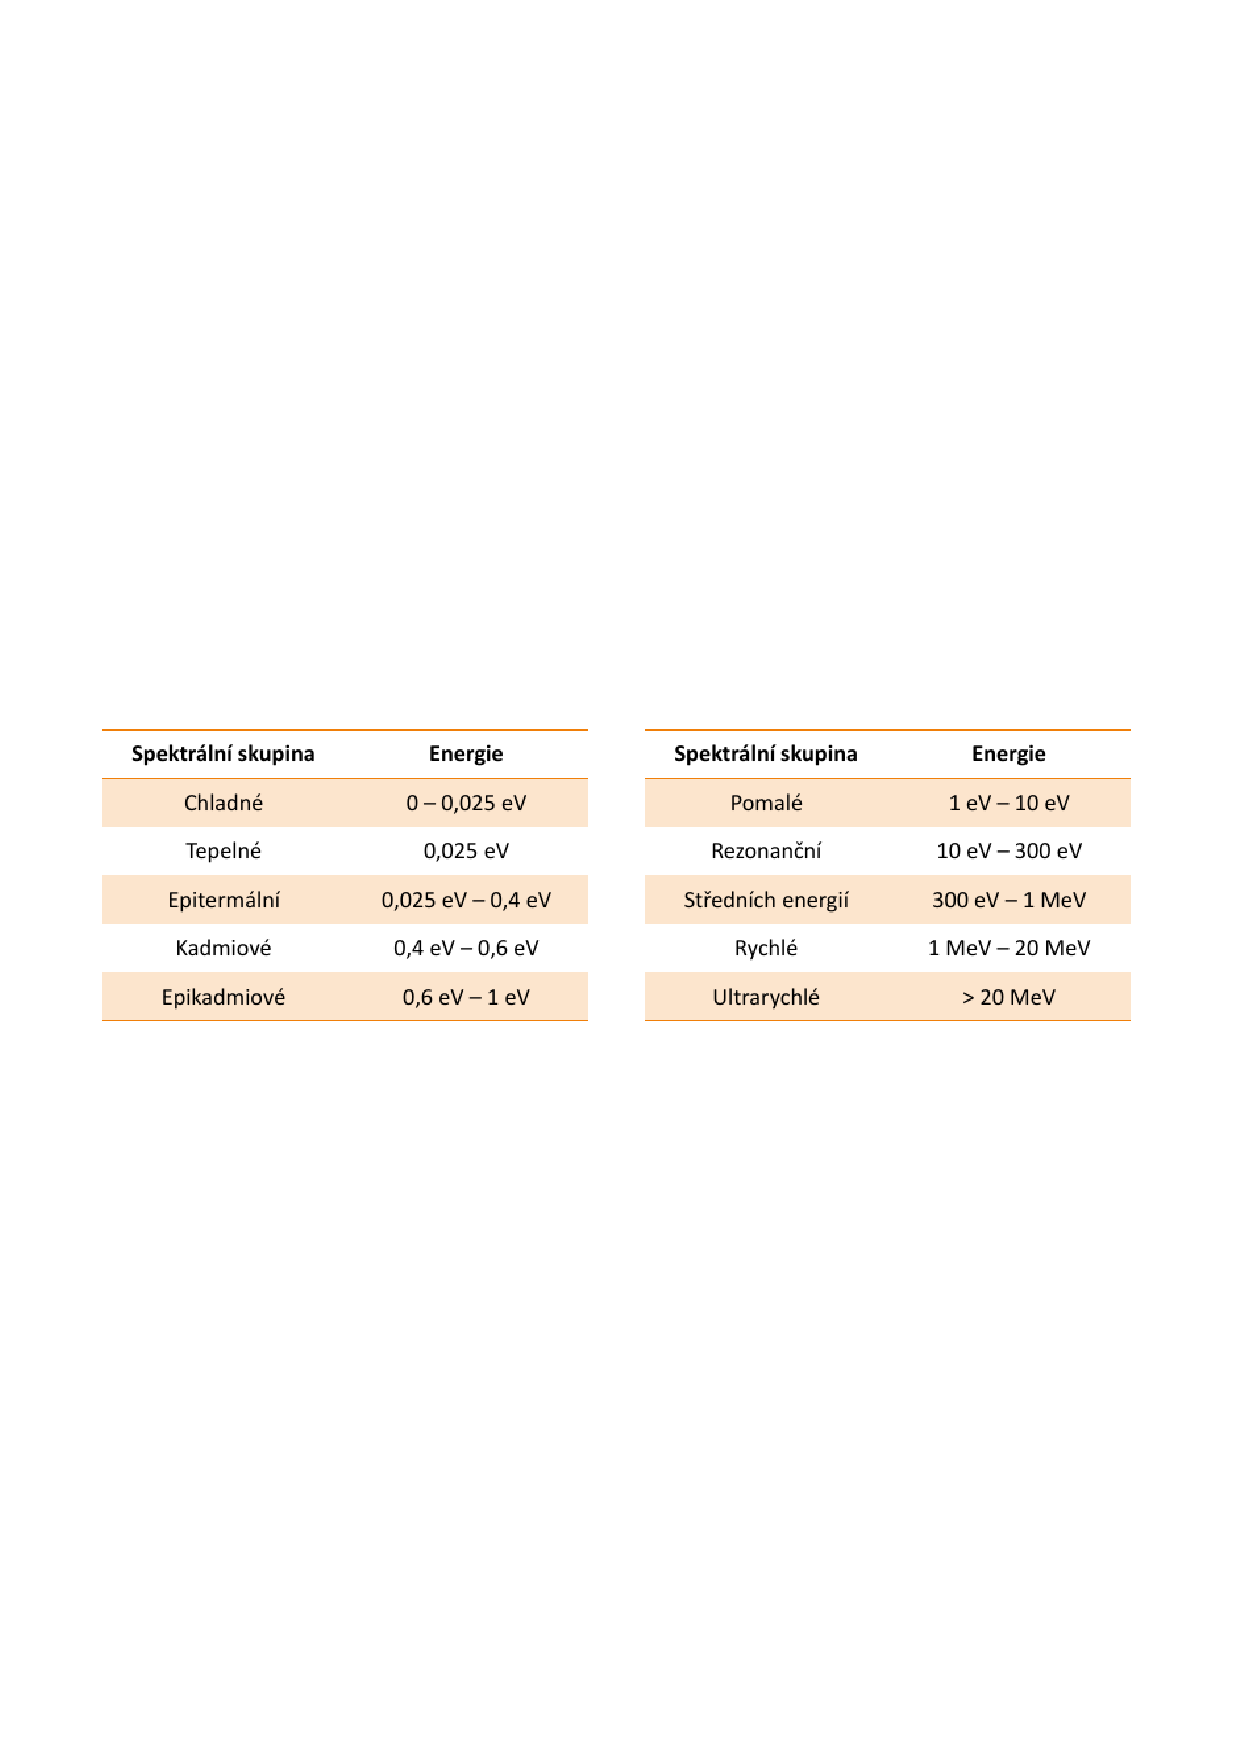
\includegraphics[width=0.8\linewidth, trim={1cm 12cm 1cm 12cm}, clip]{img/neutrony_energie.pdf}
    \caption{Rozdělení neutronů podle energie}
\end{figure}

\textbf{Měření indukované aktivity:}

\begin{itemize}
    \item Aktivita vzniklá v reakcích s neutrony $A(t)\,=\,n_{\text{R}} \cdot (1 - e^{-\lambda \cdot t})$.
    \item Může docházet k parazitním aktivačním reakcím $\rightarrow$ ovlivnění výsledků.
    \item Měření aktivity: koincidenční metodou $\beta-\gamma$ nebo počítání částíc v geometrii 4$\pi$.
    \item Rozsah většinou 10$^{10}$ až 10$^{22}$ cm$^{-2}$.
    \item Intermediální neutrony - rezonance $\rightarrow$ překryji detektor kadmiem $\rightarrow$ odfiltruji tepelné neutrony (kvůli ostrým maximům v $\sigma$).
    \item Rychlé neutrony $\rightarrow$ prahovými reakcemi.
\end{itemize}

\textbf{Počítání reakčních produktů:}

\begin{itemize}
    \item Většinou využívám (n,$\alpha$) nebo (n,p) případně (n,f) reakce.
    \item Fluence z počtu zaznamenaných částic (nutné určení účinnosti).
    \item Využívám u detektorů:
    \begin{itemize}
        \item scintilační,
        \item proporcionální počítače,
        \item štěpné komory,
        \item termoluminescenční,
        \item samonapájecí,
        \item fotografické emulze.
    \end{itemize}
\end{itemize}

\subsubsection{Detektory tepelných neutronů}

\begin{figure}[H]
    \centering
    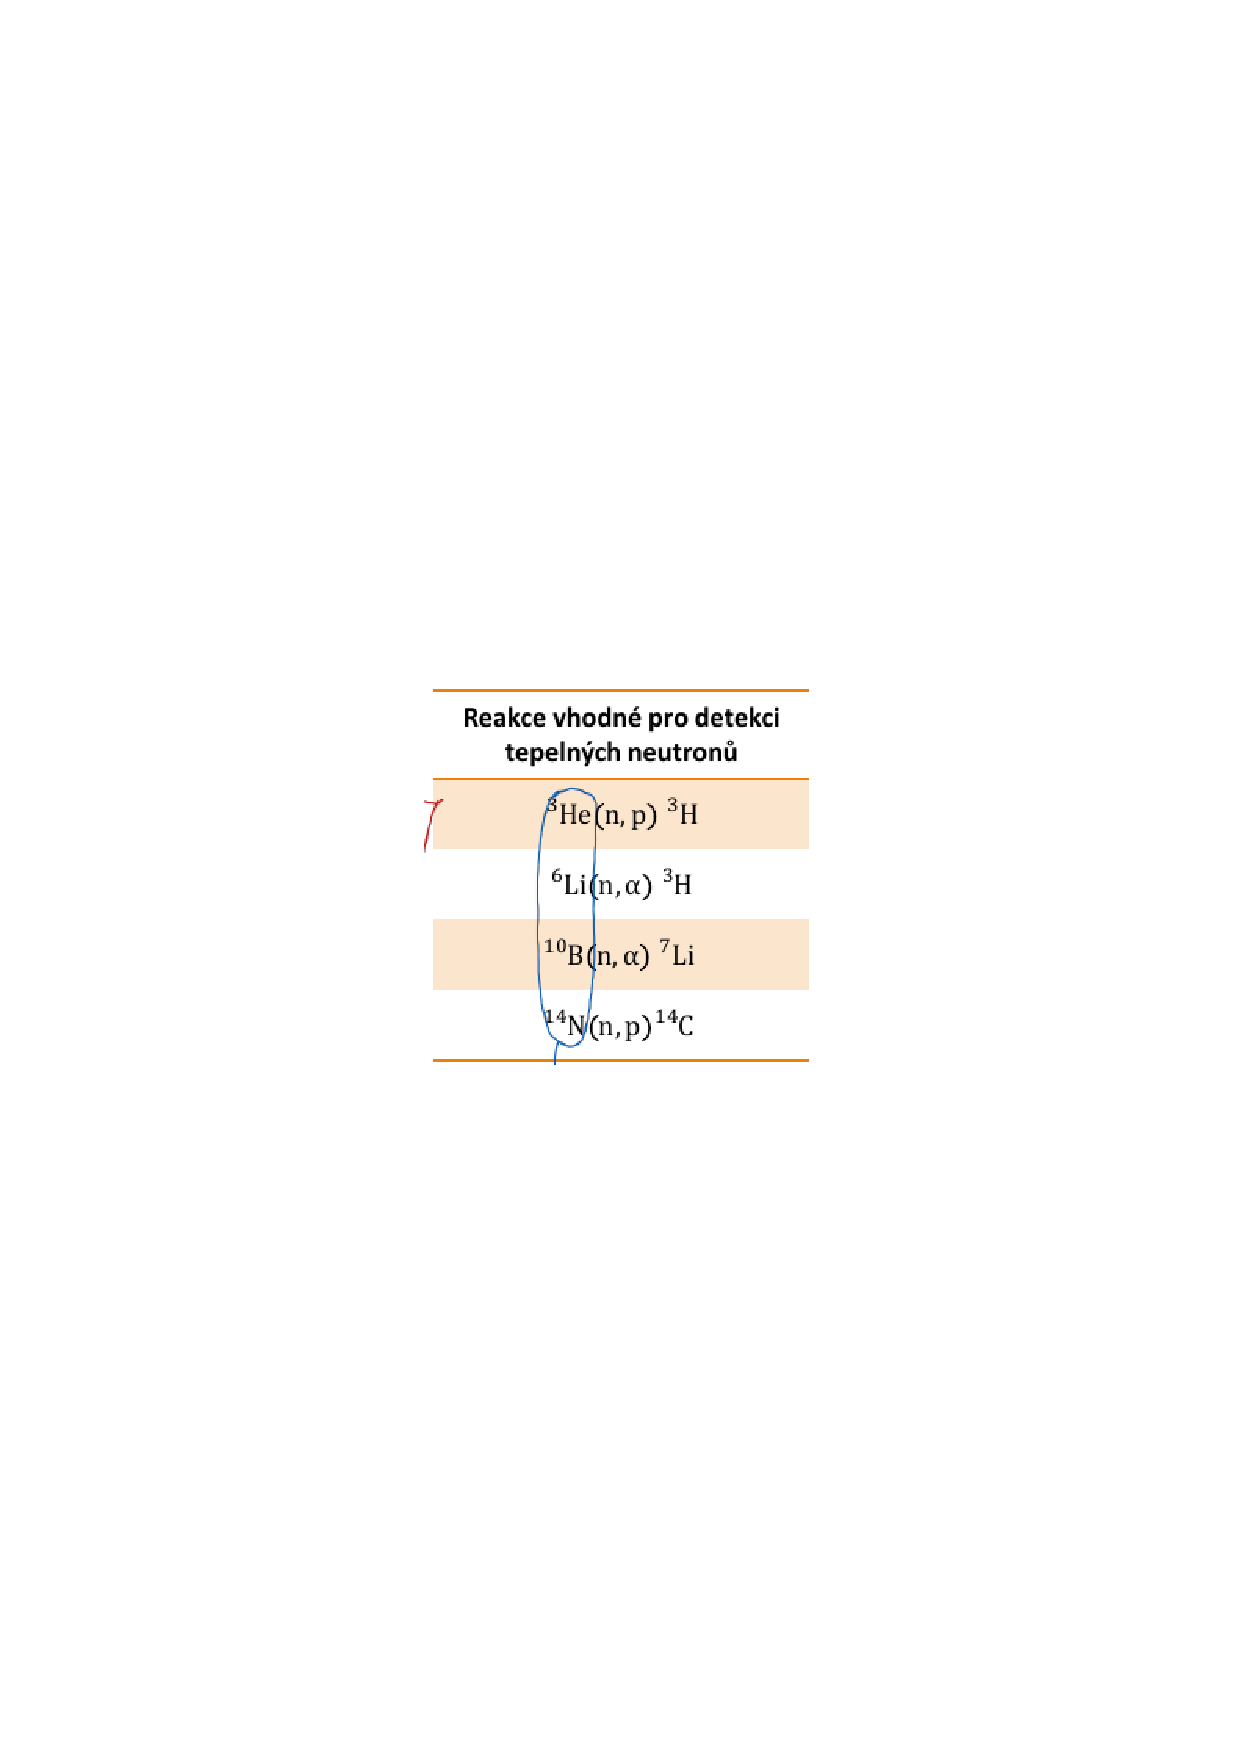
\includegraphics[width=0.4\linewidth, trim={5cm 12cm 5cm 12cm},clip]{img/reakce_tepelne_neutrony.pdf}
    \caption{Detekce tepelných neutronů -- reakce}
\end{figure}

\begin{itemize}
    \item Plynové:
    \begin{itemize}
        \item heliové a borové proporcionální komory - plynová náplň $^{3}$He a $^{10}$BF$_3$ nebo pokrytí stěny $^{10}$B,
        \item štěpné ionizační komory - stěny poryté obohaceným uranem (velká kinetická energie fragmentů),
    \end{itemize}
    \item scintilační -- konverzní materiál součástí scintilátoru (např. $^{6}$LiI(Eu)),
    \item polovodičové -- konverzní vrstva na povrchu detektoru,
    \item termoluminiscenční -- LiF obohacený o $^{6}$Li,
    \item detektory stop v pevné fázi,
    \item aktivační -- (n,$\gamma$),
    \item samonapájecí.
\end{itemize}

\subsubsection{Detektory rychlých neutronů}

\begin{itemize}
    \item Dlouhý počítač -- založeno an principu moderace.
    \item Závislost odezvy na energii nalétávající částice je "po dlouhou dobu stejná" od určité energie.
\end{itemize}

\subsection{Spektrometrie neutronů}

\begin{itemize}
    \item Většinou se používají Bonnerovy sféry.
    \item Detektor tepelných neutronů se umístí do středu PE koule s různým průměrem -- ty slouží jako moderátor.
    \item Postupně se naberou spektra.
    \item Následně $\rightarrow$ unfolding = proces, kdy je uhodnuté spektrum neutornů" jako vstup a je následně stanoveno "skutečné".
    \item Je to vleklá magie, náročné na měření.
    \item Na reaktoru používám pouze jednu bonnerku jako měřidlo dávkového příkonu.
\end{itemize}

Máme státní etalon \textbf{fluence neutronů} a \textbf{hustoty toku neutronů}.

\begin{itemize}
    \item Etalon fluence:
    \begin{itemize}
        \item zdroje neutronů: $^{252}$Cf, 1E8 s$^{-1}$ a AmBe 2E10 s$^{-1}$ a generátor 14 MeV 1E9 až 1E10 s$^{-1}$,
        \item kalibrační lavice, Bonnerův spektrometr,
        \item měřidlo prostorového dávkového ekvivalentu neutronů (to samé na VR-1 -- ta těžká bílá koule).
    \end{itemize}

    \item Etalon hustoty toku tepelných neutronů:
    \begin{itemize}
        \item grafitová prizma -- RN zdroje vkládám do moderujícího prostředí (viz neutronová laborka),
        \item vytvářím pole tepelných neutronů pro potřeby kalibrace a ověřování měřidel.
    \end{itemize}
\end{itemize}

\textbf{DOPSAT ZPRACOVÁNÍ VÝSLEDKŮ A ZDROJE NEJISTOT (ASI V JINÉ PREZENTACI)}